\chapter{Analyse der Bump-Geste}
\label{Kap3}
\label{chap:Kap3}

Bei der Bump-Geste handelt es sich um eine Interaktion bei der von einem Quellgerät, auf dem ein Anwender eine Aktivität begonnen hat, Daten durch einen Bump auf ein Zielgerät übertragen werden, damit der Anwender auf diesem seine Aktivität fortsetzen kann. Um genau zu klären, wie dieser Vorgang funktioniert, wird in diesem Kapitel untersucht, wie die Interaktion abläuft, in welchen Varianten die Geste durchgeführt werden kann, welche Endgeräte sich für die Geste eignen und wie die Geste in einer Applikation umgesetzt werden kann.

\section{Ablauf der Interaktion}
Die Interaktion kann aufgeteilt werden in die Aktionen des Benutzers und die Reaktion der Systeme auf die Interaktion.

\subsection{Aktionen des Benutzers}
Wird die Interaktion zwischen zwei Anwendern durchgeführt, halten beide Benutzer jeweils ein Gerät fest in der Hand und lassen die Geräte zusammenstoßen/bumpen. Erfolgt die Interaktion zwischen einem Anwender und einem stationären Endgerät hält entsprechend ein Anwender sein Gerät fest in der Hand und lässt es auf das stationäre Gerät bumpen.

\begin{figure}[H]
    \centering
    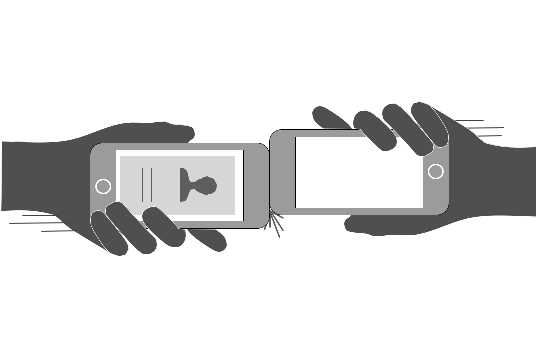
\includegraphics[width=6cm]{kapitel4/Bump.pdf}
    \label{actionUser}
\caption{Aktion des Benutzers}
\end{figure}


\subsection{Reaktion des Systems}
Die hauptsächliche Reaktion des Systems ist es, die Daten des Quellgeräts auf das Zielgerät zu übertragen und dort anzuzeigen (Siehe Abbildungen \ref{fig:transfer}, \ref{fig:anzeigen}). Die Geräte sollten aber auch eine visuelle oder akustische Rückmeldung an die Benutzer geben, um zu signalisieren, dass ein Bump von den Endgeräten festgestellt wurde, z.B. über Vibration und mit welchem Gerät/Person Daten ausgetauscht werden. 

\begin{figure}[H]
\begin{minipage}[h]{7cm}
    \centering
    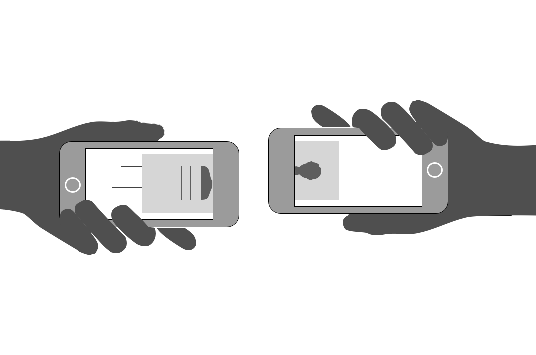
\includegraphics[width=6cm]{kapitel4/Transfer.pdf}
    \caption{Daten übertragen}
    \label{fig:transfer}
\end{minipage}
\hfill
\begin{minipage}[h]{7cm}
    \centering
    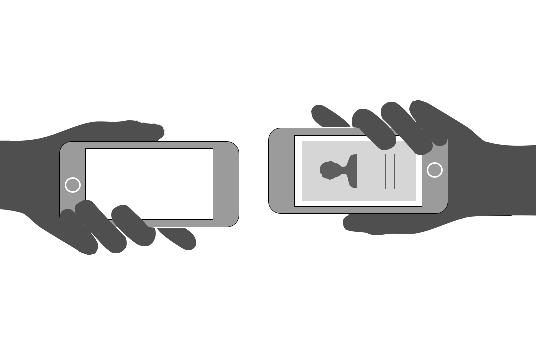
\includegraphics[width=6cm]{kapitel4/Complete.pdf}
    \caption{Daten anzeigen}
    \label{fig:anzeigen}
\end{minipage}
\end{figure}

\section{Variationen der Bump-Geste}
Die Bump-Geste lässt sich auf verschiedene Art und Weisen durchführen. An dieser Stelle sollen einige dieser Variationen als Beispiel dienen, um zu illustrieren wie eine Bump-Geste aussehen kann.

\begin{tabular}{p{5cm} p{8cm}}
    \vspace{0pt} 
    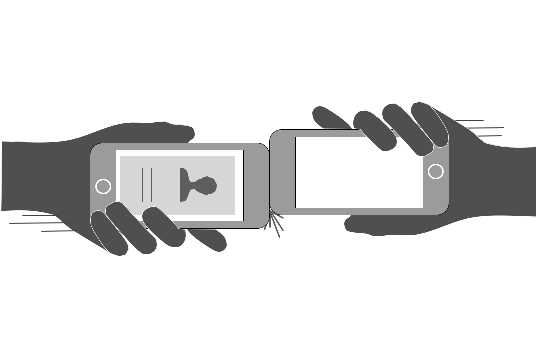
\includegraphics[width=4cm]{kapitel4/Bump.pdf}
    \begin{minipage}[h]{4cm}
        \captionof{figure}{Stirnseite an Stirnseite}    
    \end{minipage}
    & 
    \vspace{-3ex}
    \subsubsection{Stirnseite an Stirnseite}
    Die Endgeräte werden waagerecht in den Händen der Anwender gehalten und werden an den Stirnseiten zusammengestoßen.
\end{tabular}


\begin{tabular}{p{5cm} p{8cm}}
    \vspace{0pt} 
    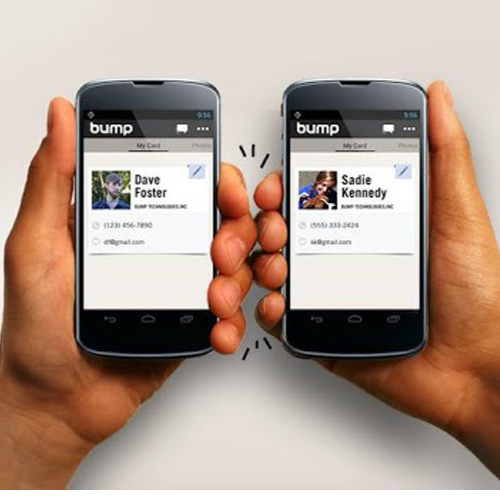
\includegraphics[width=4cm]{kapitel2/bumpPhone.png}
    \begin{minipage}[h]{4cm}
        \captionof{figure}{Längsseite an Längsseite}
    \end{minipage}
    & 
    \vspace{-3ex}
    \subsubsection{Längsseite an Längsseite}
    Die Endgeräte werden aufrecht in den Händen der Anwender gehalten und werden an den Längsseiten zusammengestoßen. Dabei können die Geräte auch von den Händen umschlossen werden wodurch die Interaktion wie ein Fistbump aussieht.
\end{tabular}


\begin{tabular}{p{5cm} p{8cm}}
    \vspace{0pt} 
    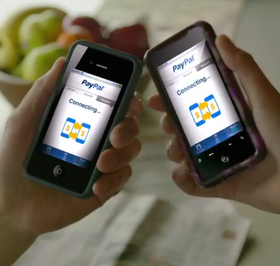
\includegraphics[width=4cm]{kapitel3/bumpEcke.png}
    \begin{minipage}[h]{4cm}
        \captionof{figure}{Ecke an Ecke}
    \end{minipage}
    & 
    \vspace{-3ex}
    \subsubsection{Ecke an Ecke}
    Die Endgeräte werden aufrecht in den Händen der Anwender gehalten und werden an den oberen Ecken zusammengestoßen.
\end{tabular}

\begin{tabular}{p{5cm} p{8cm}}
    \vspace{0pt}
    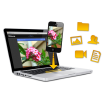
\includegraphics[width=4cm]{kapitel3/bumpLaptop.png}
    \begin{minipage}[h]{4cm}
        \captionof{figure}{Stirnseite aufstoßen}
    \end{minipage}
    & 
    \vspace{-3ex}
    \subsubsection{Stirnseite aufstoßen} 
    Ein Endgerät wird vom Anwender aufrecht in der Hand gehalten und mit der oberen oder unteren Kante auf ein stationäres Gerät (SurfaceTable, Notebook) aufgestoßen.
\end{tabular}

\section{Geeignete Endgeräte}
Aus den dargestellten Bump-Variationen ist zu erkennen, das die Bump-Interaktion zwischen verschiedenen Typen von Geräten erfolgen kann. Es gilt an dieser Stelle allgemein zu klären, zwischen welchen Geräteklassen die Bump-Geste eingesetzt werden kann. Die Geräte werden nach Terrenghi et al. \cite{Terrenghi:2009:TAM:1644246.1644265} basierend auf ihrer Bildschirmgröße kategorisiert. Die folgende Tabelle liefert einen Überblick über diese Kategorien.

\begin{table}[H]
\begin{tabular}{| >{\arraybackslash}m{4.2cm} | >{\centering\arraybackslash}m{4.2cm} | >{\centering\arraybackslash}m{4.2cm} |}
\hline
\cellcolor[HTML]{C0C0C0}Kategorie   & \cellcolor[HTML]{C0C0C0} Bildschirmgröße &  \cellcolor[HTML]{C0C0C0} Beispiel       \\ \hline
Inch size                           &  $\ge$  2,54 cm                            &  Smartphone                             \\ \hline
\cellcolor[HTML]{EFEFEF}Foot size   &  \cellcolor[HTML]{EFEFEF}  $\ge$ 30,48 cm    &  \cellcolor[HTML]{EFEFEF}Tablet         \\ \hline
Yard size                           &  $\ge$ 91,44 cm                          &  Tabletop                               \\ \hline
\cellcolor[HTML]{EFEFEF}Perch size  &  \cellcolor[HTML]{EFEFEF}  $\ge$   05 m     & \cellcolor[HTML]{EFEFEF} TV-Bildschirm  \\ \hline
Chain size                          &  $\ge$   20 m                              &  Mehrere Displays                       \\ \hline
\end{tabular}
\caption{Kategorisierung von Endgeräten}
\label{kategory}
\end{table}


Um für die Interaktion geeignete Geräte zu identifizieren gilt es erst zu definieren welche verschiedenen Rollen ein Gerät in der Interaktion einnehmen kann. Die Endgeräte können aufgeteilt werden in Quell- und Zielgeräte. Ein Quellgerät ist der Informationsträger, von welchem Daten durch den Bump auf das Zielgerät übertragen werden. Bei einem Quellgerät muss es sich um ein mobiles Endgerät handeln. Es muss vom Anwender einfach in einer oder zwei Händen gehalten, bewegt und auf das Zielgerät gestoßen werden können. Bei Zielgeräten hingegen kann es sich sowohl um ein mobiles als auch um ein stationäres Endgerät handeln. Stationäre Endgeräte zeichnen sich dadurch aus, dass Sie vom Anwender bei der Nutzung nicht in der Hand gehalten werden.

Die definierten Gerätekategorien können jetzt auf die jeweiligen Rollen aufgeteilt werden. Quellgeräte können nur Geräte aus den Kategorien Inch size und Foot size sein. Zielgeräte können zusätzlich auch aus den Kategorien Yard-, Perch- und Chain size kommen.

Nachdem die Gerätekategorien zugeordnet sind gilt, es noch zu klären, ob die Geräte aus diesen Kategorien auch für die Interaktion geeignet sind. Inch und Foot size Geräte eignen sich für die Interaktion. Sie können vom Anwender einfach geführt werden und sowohl als Quell- als auch als Zielgerät dienen. Yard size Geräte eignen sich als Zielgerät. Der Anwender kann sein mobiles Endgerät auf das Gerät aufstoßen und kann sehen, welche Auswirkungen die Interaktion auf das Zielgerät hat. Für Perch- und Chain size Geräte gilt dies nicht, da ihre Bildschirme so groß sind und der Anwender für die Interaktion so nah an den Geräten stehen muss, dass er nicht sehen kann, was auf den Zielgeräten geschieht. Geräte aus diesen Kategorien eigenen sich daher nicht gut für die Bump-Geste. 

\section{Umsetzung der Interaktion}
Um die Bump-Interaktion umzusetzen, müssen drei Teilsysteme entwickelt werden: Eines dieser Systeme muss erkennen, wenn Endgeräte angestoßen werden. Ein weiteres System muss Endgeräte identifizieren können, damit die Daten zwischen den richtigen Geräten ausgetauscht werden. Außerdem wird ein System benötigt, über das ein Kommunikationskanal zwischen den Geräten hergestellt wird, über den Daten ausgetauscht werden können.
